% das Papierformat zuerst
\documentclass[a4paper, 11pt]{article}

\usepackage[utf8]{inputenc} % Kodierung
\usepackage[ngerman]{babel} % Sprache
\usepackage{graphicx}  % Bildchen
\usepackage{float}  % Bildchen2
\usepackage{rotating} %Bildchen3

% wir wollen auf jeder Seite eine Ueberschrift
\pagestyle{headings}

% hier beginnt das Dokument
\begin{document}

\thispagestyle{empty}
\begin{center}
\Large{Karlsruher Institut für Technologie}\\
\end{center}

\begin{center}
\Large{Fakultät für Wirtschaftswissenschaften}
\end{center}
\begin{verbatim}





\end{verbatim}
\begin{center}
\textbf{\LARGE{Seminararbeit}}
\end{center}
\begin{verbatim}


\end{verbatim}
\begin{center}
\textbf{am Institut für Angewandte Informatik und Formale Beschreibungsverfahren}
\end{center}
\begin{verbatim}


\end{verbatim}

\begin{verbatim}









\end{verbatim}
\begin{flushleft}
\begin{tabular}{lll}
\textbf{Thema:} & & Linked Open Data basierte Web 3.0 Anwendungen \\
& & \\
& & \\
\textbf{eingereicht von:} & & Xinji Du\\
& & Christoph Gielisch \\
& & Andreas Gutzan \\
& & Clemens Stolle \\
& & \\
\textbf{eingereicht am:} & & 13. Juli 2011\\
& & \\
\textbf{Betreuer:} & & Herr Prof. Dr. Rudi Studer \\
& & Herr Dipl.-Wirt.-Ing. Daniel Herzig \\
& & Herr Dipl.-Inf. Benedikt Kämpgen \\
& & Herr Dipl.-Inf. Günter Ladwig
\end{tabular}
\end{flushleft}

\begin{abstract}Das Internet umfasst eine riesige Menge an Informationen jeglicher Art. Da diese aber meist in einer unstrukturierten Weise vorliegen, ist es schwierig Daten aus verschiedenen Quellen miteinander zu verknüpfen. Hier soll Linked Open Data Abhilfe schaffen. Durch diverse Beschreibungs- und Abfragesprachen können Informationen strukturiert und standardisiert gespeichert und abgefragt werden. Dadurch wird die maschinelle Informationsverarbeitung erheblich vereinfacht.\\\\
Eurotrip ist ein Allgemeinwissen- und Geographiequiz, das mehrere Linked Open Data Datensätze verwendet um immer unterschiedliche Fragen zu generieren. Da dem Spiel kein fester Fragenkatalog zu Grunde liegt, existiert theoretisch eine unbegrenzte Anzahl an Fragemöglichkeiten. Es werden über spezielle Abfragen mehrere Quellen so miteinander verknüpft, dass eine Frage-Antwort Kombination mit Bildern, Texten und geographischen Daten entsteht, die es in dieser Form noch nicht gibt.\\\\
Mit jeder Frage generiert der Spieler einen neuen Datensatz für einen Ort, der Informationen wie lokale Sehenswürdigkeiten, dazugehörige Fotos, die Landesflagge und Verweise auf andere Linked Open Data Ressourcen enthält. Dieser Datensatz wird in strukturierter Form gespeichert, so dass eine spätere Weiterverwendung der neu verknüpften Daten durchaus denkbar ist. \\\\
In spielerischer Form wird so die Linked Open Data Wolke mit neuen Querverweisen und Informationsverknüpfungen angereichert.
\end{abstract}
\thispagestyle{empty}
\newpage
\tableofcontents
\setcounter{page}{1}
\pagenumbering{Roman}

\newpage
\setcounter{page}{1}
\pagenumbering{arabic}
\section{Einleitung}
\subsection{Problemdefinition}
Neben einer Vielzahl von unstrukturierten Daten entsteht im World Wide Web eine große Wolke mit frei verfügbaren Daten,  die per URI (Uniform Resource Identifier) kodiert und verlinkt sind. Diese Linked Open Data (LOD) sind Teil des Semantic Web und besitzt gegenüber konventioneller Datenrepräsentation viele Vorteile.\\\\
Das folgende Projekt entsteht in Gruppenarbeit als Teil des Seminarpraktikums „Web 3.0 – Linked Open Data Applications“. \\\\
Es hat das Ziel einen lauffähigen Prototyp einer LOD Anwendung zu erstellen, der mindestens zwei LOD Datensätze verwendet und dessen Verwendung einen direkten Nutzen aus diesen Datensätzen zieht. Das Ergebnis soll so flexibel gehalten werden, dass weitere Datensätze potentiell integriert werden können. 
\subsection{Herangehensweise und Ziele}
Im Folgenden wird sowohl die Beschreibung  der Projektidee als auch die technische Umsetzung geschildert. Ebenso wird kurz auf die Projektplanung eingegangen. Der Fokus liegt speziell auf der Evaluierung der Vorteilhaftigkeit bei der Verwendung von Linked Open Data. \\\\
Die Projektidee muss innovativ und gleichzeitig im technischen sowie zeitlichen Rahmen realisierbar sein. Das Ziel soll primär auf der Verwendung von mehreren LOD Datensätzen liegen, deren Benutzung die Vorteile von LOD Datensätze ermöglicht. Des Weiteren wird Wert auf die flexible Erweiterungsmöglichkeit gelegt. \\\\
Dem Projektteam ist bewusst, dass das Ergebnis kein marktfähiges Produkt sondern lediglich ein Prototyp darstellen kann. Einbußen bei der Bedienerfreundlichkeit, Geschwindigkeit sowie Fehlerfreiheit werden notwendigerweise in Kauf genommen. Schwächen und Schwierigkeiten bei der Verwendung von LOD werden explizit den Stärken gegenübergestellt.\\\\
Dieser Arbeit liegt eine CD bei, die den Quellcode des kompletten Projektes beinhaltet.
\newpage
\section{Beschreibung der Idee}
\subsection{Anwendungszenario}
Für die Anwendbarkeit des Programmes gilt es zunächst zwei verschiedene Grundüberlegungen zu separieren. Es stellt sich die Frage, welchen Nutzen das Produkt zum einen für den potentiellen Anwender, also den Spieler, und zum anderen für den Entwickler bzw. den Vertreibenden bietet.\\\\Für den Anwender ist das Programm ein Quiz- oder Lernspiel. Abgefragt werden hauptsächlich geografische Kenntnisse. Dabei sorgt eine Punktevergabe für einen kompetitiven Faktor. Das Spiel positionier sich somit sowohl als Edutainment-Software\footnote{http://www.hdm-stuttgart.de/ifak/medientipps/edutainment/definition/} als auch als Unterhaltungssoftware für die kurzweilige Ablenkung, z.B. als Facebook-Spiel.\\\\
Als Anbieter der Software ist neben der Schaffung einer Einnahmemöglichkeit über Werbeeinblendungen oder Verkauf der Software vor Allem die Generierung von strukturierten Daten interessant. 
\subsection{Spielablauf}
Der Spielablauf gliedert sich in zehn Fragerunden. In jeder Fragerunde sucht das Programm drei Fotografien zu einer europäischen Stadt, die gewissen Ansprüchen genügen muss\footnote{siehe getCity.php in Kapitel \ref{sec:getCity}}, heraus. Der Spieler muss nun versuchen diese Stadt mit Hilfe der Fotografien zu erkennen und sie auf einer Europakarte mit einem Mausklick möglichst genau zu lokalisieren. Er bekommt dabei weniger Punkte je weiter sein Tipp vom richtigen Zielort entfernt liegt, wobei ab einer gewissen Entfernung pauschal null Punkte vergeben werden.\\\\ Weiterhin kann er sich nach Bedarf in jeder Fragerunde im Tausch gegen Punkte drei neue Fotografien oder auch einen 200 Zeichen langen Kurzhinweis anzeigen lassen. Wenn der Spieler mit seinem Tipp eine gewisse Maximalentfernung nicht überschreitet bekommt er darüber hinaus eine Bonusfrage zur aktuellen Stadt oder deren Land gestellt. Diese vermittelt zusätzliche Hintergrundinformationenund gibt dem Spieler die Möglichkeit ein paar Bonuspunkte zu erspielen.\\\\ 
Die so in einer Fragerunde erspielten Punkte werden kumuliert. Ziel des Spiels ist es nach zehn Fragenrunden einen möglichst hohen Punktestand zu erreichen.
\subsection{Alleinstellungsmerkmal und Abgrenzung}
Die grundlegende Spielidee wurde so schon in Facebook- sowie iPhone-Apps implementiert\footnote{http://www.facebook.com/apps/application.php?id=134046623315935, \\http://itunes.apple.com/de/app/georific/id320207678?mt=8}. Allerdings setzen diese zur Erzeugung der Fragen auf statische Datenbanken und sind somit im Fragenumfang limitiert. Durch den Einsatz von Linked-Open-Data konnte hier eine dynamische, sich selbstständig aktualisierende Variante geschaffen werden. Desweiteren sorgt der Aufbau des Programmes, gerade in Bezug auf die Bonusfragen, für eine modularisierte Erweiterbarkeit des bestehenden Programmes mit anderen Datenquellen im Semantic Web.\\\\
Dazu kommt, dass das Programm keinerlei Anforderungen an den Nutzer stellt, wie die Wahl eines geeigneten Betriebssystems oder einen eingerichteten Account auf der Website. Lediglich ein aktueller Browser wird benötigt.
\subsection{Semantic Gaming}
Dieser Abschnitt gibt einen kurzen Überblick über den Begriff des Semantic Gaming und beschreibt, welche Teile davon für uns von Interesse sind. Die genaue technische Umsetzung findet sich in Kapitel \ref{sec:gen-struk-daten}.\\\\
Ein grundlegendes Problem des Semantic Webs ist die, verglichen mit anderen Web 2.0 Anwendungen, relativ geringe Nutzerbeteiligung.  Es benötigt diese allerdings, da das Strukturieren der Daten ein Vorgang ist, der zumeist nicht einfach automatisiert werden kann, sondern durch Menschen geschehen muss. Derjenige, der die Daten strukturiert, zieht aber häufig erstmal keinen direkten Nutzen daraus. Zu hoffen, dass das Strukturieren durch reinen Altruismus oder die Bezahlung in irgendeiner Art und Weise befriedigend erfolgt, erscheint wenig vielversprechend. An dieser Stelle setzt das System der \textit{Games with a Purpose for the Semantic Web}\footnote{http://www.computer.org/portal/web/csdl/doi/10.1109/MIS.2008.45} an. Es setzt darauf dem Nutzer bzw. in diesem Fall dem Spieler für das Strukturieren der Daten einen Gegenwert in Form von Spielspaß und einer Art intellektuellen Wettbewerb zu geben.\\\\
Diese Strukturierung der Daten passiert dabei bei uns unbewusst und im Hintergrund, um den Nutzer nicht aus der Immersion des Spiels zu reißen. Für ihn soll zu jedem Zeitpunkt die Unterhaltung durch die Software im Vordergrund stehen. 
\newpage
\section{Projektplanung}
\subsection{Arbeitspakete und Zuständigkeiten}
Innerhalb des Teams wurde zunächst das Ziel formuliert sowie analysiert, welche Möglichkeiten LOD Datensätze bieten. Als Kommunikationsplattform hat sich das Projektteam bewusst auf ein regelmäßiges, wöchentliches Treffen verständigt. Dies diente der Projektplanung, zeitlicher und inhaltlicher Kontrolle sowie der Abstimmung und Zusammenführung individuell erarbeiteter Teilmodule.\footnote{Eine grundlegende Übersicht über die Arbeitspakete des Projekts lässt sich aus Abbildung 1 im Anhang unter Abschnitt \pageref{pic:Pakete} entnehmen.}\\\\
Innerhalb des Projektteams wurde für jede Aufgabe Milestones mit Fristen definiert und einer Person direkt zugeordnet.\footnote{Ein Auszug der Liste mit Arbeitspaket, Milestones, Frist und Zuständigkeit ist in der Zwischenpräsentation enthalten.}
\subsection{Evaluierung}
Als vorteilhaft hat sich herausgestellt keine absolute Frist für die Projektidee zu setzen. Aufgrund von Schwierigkeiten mit LOD Datensätzen musste die Idee inkrementell angepasst werden. Die Trennung in Klassen ermöglichte die parallele Ausarbeitung, die mit dem Versionsverwaltungstool Github  effizient ermöglicht wurde. Da trotzdem viel Abstimmung nötig war, stellte das wöchentliche Treffen das Kernelement der Projektdurchführung dar.  Die Aufnahme des Arbeitspakets „Organisation“ war maßgeblich für die effiziente und erfolgreiche Projektkontrolle verantwortlich. Für unseren Einsatzzweck hat sich das Treffen als effektiveres Mittel herausgestellt als eine zu zeitlich determinierte Gesamtplanung innerhalb eines Projektplanungstools.\\\\
Die Unausgeglichenheit der Projektaufgaben aufgrund unterschiedlicher Ausgangspositionen stellte zunächst eine Schwierigkeit dar. Durch klare Verhaltensregeln, spezifische Einarbeitung sowie die Anpassung der Aufgaben an das vorhandene Know-how ist diese Situation nachhaltig verbessert worden.
\newpage
\section{Umsetzung, Softwarepakete und Programm}
\subsection{Schematischer Aufbau}
Konzeptionell baut das Programm auf einer zentrierten Struktur auf. Dabei ist die Javascript-Engine das Herz der Anwendung. Sie kann auf verschiedene PHP-Dateien zugreifen, die sie quasi wie Methoden benutzt. Die PHP-Dateien hingegen realisieren die Abfragen der LOD-Datensätze. Somit benutzt die Engine reines JSON als Schnittstelle, wohingegen die PHP-Dateien die verschiedenen Schnittstellentechnologien der Datensätze verwendet und zumeist die gefundenen Daten für die Engine aufbereitet. Durch die sehr dynamische, heterogene Entwicklung des Semantic Webs ist ein Wechsel der Datensätze oder des Abfragemodus eine realisitsch auftretende Problematik. Das Design hat hier den Vorteil, dass bei gleichbleibenden Schnittstelle zwischen Engine und PHP-Datei diverse Änderungen bei der Abfrage von Datensätzen realisiert werden können, ohne dass die eigentliche Engine angepasst werden muss.\footnote{Eine vollständige Konzeptskizze ist im Anhang unter Abschnitt \pageref{pic:Konzept} zu finden}\\\\
Die implementierten PHP-Klassen sind im Detail:
\begin{itemize}
\label{sec:getCity}
\item \textbf{getCity.php:} Durchsucht Geonames mit gewissen Filterkriterien nach Städten. So wird nach europäischen Städten mit mehr als 400000 Einwohnern gesucht\footnote{Für Deutschland wird dieser Filter auf 250000 abgesenkt}, die nicht in Russland oder der Ukraine liegen.
\item \textbf{getPictures.php:} Die Engine übergibt dieser PHP-Datei einen validen\footnote{siehe check.php } Stadtnamen. Zu diesem sucht die getPictures dann in der Freebase nach passenden Sehenswürdigkeiten, checkt in der DBpedia ob zu diesen FlickrWrappr-Photocollections existieren und holt sich aus diesem dann zu je drei Sehenswürdigkeiten mit Collection je zwei Fotografien. Diese werden dann, zusammen mit den DBpedia- und FlickrWrappr-Verlinkungen an die Engine zurückgegeben.
\item \textbf{getInfo.php:} Holt sich den englischen Abstract der übergebenen Stadt, kürzt ihn auf knapp 200 Zeichen, wobei eine mittige Textstelle ausgewählt wird und gibt diesen String als Ergebnis für den Kurzhinweis zurück.
\label{sec:check}
\item \textbf{check.php:} Diese Datei prüft ob ein übergebener URI ein existierender Bezeichner für einen DBpedia-Eintrag ist. Dies wird benutzt, um ein Grundmaß an Validität bei der Übergabe von Resourcen via URI zu gewährleisten.
\item \textbf{getFlag.php:} Eine Beispielimplementierung für eine Bo"-nus"-fra"-gen"--Me"-tho"-de. Diese sollen immer drei Länder übergeben bekommen und zu diesen drei Antwortmöglichkeiten ausgeben. Dies vollführt diese Datei mit Hilfe des Flaggen-Thumbnails der Länder bei der DBpedia.
\end{itemize}
\subsection{Verwendete Technologien und Frameworks}
Neben dem Linked-Open-Data Ansatz des Semantic Web benutzt das Programm selbst noch weitere Technologien und Frameworks.\\\\
Auf der Clientseite läuft im Browser einer Webapplikation deren Benutzeroberfläche mit HTML, CSS und JavaScript realisiert wurde. In Javascript (mit der jQuery Bibliothek\footnote{http://www.jquery.com}) ist auch die eigentliche Engine geschrieben, die das Spielgeschehen steuert und die Programmteile miteinander verbindet. Das Kartenmaterial wird über die Google Maps API\footnote{http://code.google.com/intl/de/apis/maps/} eingebunden. Mit Hilfe dieser API wird auch die Entfernungsberechnung anhand des vom Spieler angeklickten Ortes durchgeführt. Zur Kommunikation zwischen den Programmteilen wird auf das JSON Format gesetzt. Serverseitig fungieren PHP Skripte als Datenprovider. Diese fragen die verschiedenen Datensätze ab und filtern eventuell die Ergebnisse. Die Anwendung ist somit auf jedem Webserver mit PHP Unterstützung lauffähig. Während der Entwicklung nutzten wir das XAMPP Paket\footnote{http://www.apachefriends.org/de/xampp.html} welches den Apache Webserver mitliefert.
\subsection{Verwendete LOD-Datensätze}
Die verwendeten LOD-Datensätze sind:
\begin{itemize}
\item \textbf{Geonames} wird eingesetzt, um eine Auswahl an Städten zu erzeugen, die der Spieler später dann lokalisieren muss. Diese Datenquelle wurde gegenüber der DBpedia bevorzugt, da hier die Städte klarer strukturiert abgespeichert sind. So fällt die Abfrage der Städte und die Länder in denen diese liegen leichter, da es hier eine eindeutige Hierarchie von Kontinent, Land und Stadt gibt. 
\item Die \textbf{DBpedia} wird gleich an mehreren Stellen im Programm verwendet. Grundsätzlich gilt, dass wenn Namen von Städten, Ländern oder Sehenswürdigkeiten zwischen verschiedenen Programmteilen ausgetauscht werden, dass diese dann mit ihrem DBpedia URI übergeben werden müssen, um die Validität zu gewährleisten. Weiterhin werden sowohl der Kurzhinweis als auch die (implementierte) Bonusfrage mit Hilfe der DBpedia generiert. Auch wird dort mit dem dafür zuständigen Tag geprüft, ob eine Sehenswürdigkeit oder Stadt eine FlickrWrappr-PhotoCollection besitzt.
\item \textbf{Freebase} dient vor Allem der Optimierung der Foto-Suchergebnisse. Da sich rein mit einer Stadt getaggte Bilder als teilweise ungenügend herausgestellt haben, wird Freebase zunächst nach bekannten touristischen Sehenswürdigkeiten der einzelnen Städte abgefragt, da zu diesen i.d.R. aussagekräftigere Fotos zu finden sind.
\item Der \textbf{Flickrwrappr} basiert auf einem PHP-Skript der FU Berlin. Man übergibt diesem Skript als Übergabeparameter einen Stadt- oder Sehenswürdigkeitsnamen, welcher dem URI der DBpedia entsprechen sollte. Der Flickrwrappr gibt als Sucherergebnis strukturierte Daten in Form einer XML/RDF Datei zurück, aus der die Links zu den gesuchten Bildern extrahiert werden können.
\item Im Zuge der Bonusfrage können außerdem noch \textbf{weitere Datensätze} in das bestehende Programm integriert werden. Solange diese die gleiche Schnittstelle wie die existierende Bonusfrage benutzen, können sie ohne weitere Probleme in das Programm integriert werden.
\end{itemize}
\subsection{Stabilität und Verfügbarkeit}
Das Programm an sich läuft trotz seines Prototypen-Status recht stabil. Allerdings ist die Erreichbarkeit von drei Datenquellen für den grundlegenden Ablauf der Fragerunden zwingend erforderlich. Diese sind Geonames, die DBpedia sowie der Flickrwrappr. Ein Ausfall der Freebase würde lediglich die Qualität der Bilder senken, da dann das Heraussuchen von Touristischen Attraktionen wegfallen würde. Sollte einer der Datenbanken der Bonusfragen nicht antworten, wäre ein Fallback auf eine andere Bonusfrage oder das komplette Deaktivieren denkbar. Bei beiden Möglichkeiten ist weiterhin ein stabiler, wenn auch eingeschränkter Betrieb des Programms möglich.\\\\ 
Nach unseren Beobachtungen war Geonames nahezu immer erreichbar, wäh"-rend bei DBPedia temporäre Ausfälle zu verzeichnen waren. Der Flickr"-Wrappr funktionierte die meiste Zeit problemlos, wenn auch sehr langsam. Ende Juni allerdings war er schlagartig nicht mehr erreichbar, was laut seinem Entwickler auf wiederholte Botattacken zurückzuführen ist. Er empfahl uns eine lokale Kopie seines Programmes zu verwenden, was wir von da an taten.
\subsection{Generierung strukturierter Datensätze}
\label{sec:gen-struk-daten}
Ein weiterer technischer Aspekt ist die Generierung eigener strukturierter Daten. Dies ist einer der Grundgedanken sowohl des Semantic Webs als auch des Semantic Gamings. Unser Programm ist dabei in der Lage schon rudimentär neu von uns verknüpfte Daten in Kombination mit Daten, die wir durch die Eingabe der Nutzer gewonnen haben, als strukturierte Daten abzuspeichern. Dabei wird für jede Stadt jeweils ein XML-Datensatz angelegt, der dann befüllt wird mit den aktuellen Sehenswürdigkeiten, Bildlinks sowie der vom Nutzer bei genau dieser Kombination erreichten Entfernung zum Zielort.\\\\ Dadurch erschaffen wir eine Datenbank aus der man durch geschicktes Abfragen eine ganz neue Qualität an Information beziehen kann. So sind wir in der Lage bei ausreichend großen Nutzerdateninput durch gemittelte Entfernungen Aussagen über den Bekanntheitsgrad von Städten im Allgemeinen, aber auch deren Sehenswürdigkeiten zu treffen. Denkbar wäre z.B. auch das Blacklisting einzelner unrelevanter Bilder, die eine signifikante Abweichung zu anderen Bildern der gleichen Sehenswürdigkeit etc. aufweisen.\\\\
Wir sind damit in der Lage das bei LOD grundlegend heikle Thema der Bewertung von Elementen innerhalb einer Cloud zu verbessern, da man nun mit der Entfernung zumindest ein Maß für die Bekanntheit dieser Städte und Sehenswürdigkeiten besitzt.\\\\
In Eurotrip generiert so jeder Spieler genau die Daten, die wir zu Beginn der Entwicklung gesucht haben, welche aber in der Form noch nicht vorhanden waren. Dies dürfte dem Grundgedanken des Semantic Webs entsprechen, da dieses seine Mächtigkeit ja gerade durch die nahezu unendliche Möglichkeit der Kombination und Verknüpfung von bestehenden und das Einpflegen von neuen strukturierten Daten bezieht.
\subsection{Installation und Betrieb}
Das Spiel selbst benötigt keine clientseitige Installation. Einzig ein funktionierender, aktueller Browser\footnote{getestet in Internet Explorer 9, Firefox 3.5+, Google Chrome 11+, Safari 5}, der in der Lage ist Javascript auszuführen, ist von Nöten. Der Start erfolgt durch Ansteuerung der Webadresse.\\\\
Für den Betrieb des Spiels ist der Anbieter des Programms allerdings gezwungen einen Webserver zu betreiben. Dieser muss in der Lage sein PHP-Code zu interpretieren und so die nötigen Abfragen auf die verschiedenen Datenquellen auszuführen.
\newpage
\section{Lessons learned}
\subsection{Erkenntnisse}
Das wichtigste Ergebnis unserer Projektarbeit ist, dass eine Spiel-Anwendung mit LOD Datensätzen machbar ist. Insbesondere ist es möglich, ohne dass die positiven Eigenschaften eines Spiels vernachlässigt werden. Auch als Prototyp kann die Anwendung dem Benutzer richtig Spaß machen.\\\\
Für die Anwendung als Spiel macht der Einsatz von LOD dort am meisten Sinn, wo strukturierte Datenabfragen gefragt sind. Besonders bei Spielideen mit Wissensabfragen (Lernspiele…) ist das der Fall. Umgekehrt macht die Spielanwendung für LOD Daten Sinn, wenn die Benutzer mit Spaß am Spiel dazu beitragen, strukturierte Daten zu generieren. Aus Ergebnissen, Reaktionen des Benutzers, gesammelte Datenverlinkungen etc. kann durch die Anwendung ein Mehrwert entstehen. Im Falle dieses Spiels „erzeugt“ das spielen eine neuartige Cloud mit Städtenamen, denen Sehenswürdigkeiten, Bilder, Nationalflaggen und weitere Daten aus verschiedenen Datenbanken zuordenbar sind und sogar Aussagen zu deren Relevanz (Erkennungs- und Bestimmungsgrad im Spiel) getroffen werden. Dies ist äußerst relevant, denn bei der Nutzung von LOD sind wir des Öfteren auf das Problem der Relevanz, Priorisierung etc. gestoßen.\\\\
Grundsätzlich entsteht dann ein Mehrwert, wenn verschiedene Datenbanken effizient miteinander verknüpft und  gekoppelt werden. Die Effizienz der LOD Nutzung lässt sich erhöhen, indem man vom separaten „realtime lookup“ zum konsequenten  „Abwandern“ von Verlinkungen übergeht.  So sind wir von der getrennten Abfrage von Sehenswürdigkeiten und Bildern auf eine verbundene Abfrage übergegangen, in der der Link von Freebase zu DBpedia und von dort weiter zur Flickr Photo Collection führt. Leider sind diese Wege nicht immer konsistent verfügbar. Auch für dieses Problem kann der Output unserer Anwendung Abhilfe schaffen.\\\\
Die technischen Voraussetzungen sind relativ leicht erlernbar, wenn Vorwissen in Programmiersprachen (wie Java, C++ etc.) verfügbar steht. Angenehm ist, dass der Technologieeinsatz sehr flexibel ist und so gut an die Know-how- Verfügbarkeit des Teams angepasst werden kann. Die Verwendung von PHP für die Programmierung der Klassen hat sich als sehr gute Wahl herausgestellt, da die Einarbeitung im verfügbaren Zeitrahmen möglich war. Bei der Zusammenführung und im Umgang mit Fehlern hat es sich als hilfreich erwiesen, Projektmitglieder mit ausreichendem Vorabwissen im Team zu haben. Die Kombination von Javascript, AYAX und PHP erwies sich als kompatibel und funktionsfähig. Erschwerend war der Umgang mit den uneinheitlichen Standards bezüglich der Abfragemethode (Sparql, Jason, XML). \\\\
Bei der technischen Umsetzung im Team war die frühe Einigung auf Schnittstellenformate und Übergabeparameter für die Übersichtlichkeit maßgeblich verantwortlich. Ebenso das Versionsverwaltungstool Github. Im Verlauf der Zusammenarbeit identifizierten wir folgende 3 drei Faktoren als ausschlaggebend für den Erfolg: uneingeschränktes Kommittent und Verantwortungsbewusstsein, aktives Nachfragen im Fall von Unklarheiten sowie kontinuierliche Kontrolle des Projektfortschrittes.  \\\\
Wie erwartet (und in der Planung berücksichtigt) wurde für Feinabstimmung (Umgang mit Sonderzeichen, Leerzeichen oder Anführungszeichen in Abfragen etc. …) und Tests am Abschluss viel Zeit verwendet. 
\subsection{Vor- und Nachteile von Linked Open Data}
In diesem Kapitel werden die Erfahrungen unseres Projektteams mit dem Umgang mit LOD Datensätzen evaluiert. Diese Aussagen beziehen sich dabei gezielt auf jene Datensätze, die wir für unser Spiel benutzt haben. \\\\
\textbf{Vorteile:}
\begin{itemize}
\item Linked Open Data sind open source und somit kostenlos für jedermann verfügbar. Eine schnell wachsende Datenmenge bietet Informationen in diversen Quellen zu einer Vielzahl verschiedener Themen. Kein abgeschlossenes System wäre in der Lage in dieser Geschwindigkeit zum Wissenszuwachs beizutragen (n-n Beziehung). Durch die dezentrale Speicherung ist das Datenvolumen nahezu unbegrenzt. Bei der Benutzung von LOD sind geringe Eintrittsbarrieren zu überwinden, da die „Ansteuerung“  leicht erlernbar sowie der Technologieeinsatz flexibel gestaltet werden kann. 
\item Im Gegensatz zu konventioneller Informationsrepräsentation ermöglicht die Semantik eine strukturelle Kategorisierung. Als Beispiel erlaubt der Übergang von wikipedia.org auf dbpedia.org eine Abfrageform hinsichtlich der gewählten Hierarchie.  Durch Querverlinkungen zu verwandten, bereits existierenden Daten sind alle LOD miteinander verknüpft. Durch das „abwandern“ dieser Links entsteht ein optimaler Zugang zu allen verfügbaren Daten, die für verschiedenste Anwendungen genutzt werden können.
\item Die Verantwortung der Datenpflege liegt beim Benutzer. Falls die in diesem Projekt generierten Outputdaten online verfügbar gestellt wür"-den, könnte es das LOD Netz erweitern. Die Kombination von Geo"-names-Städtelinks, DBpedia-Einträgen, Freebase-Informationen zu Sehens"-würdigkeiten und die Ergebnisse des Nutzerverhaltens bezüglich des Erkennungsgrad der gewählten Bilder stellt einen neuartigen Mehrwert dar, der anderen Nutzern zur Verfügung gestellt werden kann.
\end{itemize}
\textbf{Nachteile:}
\begin{itemize}
\item Dezentrale Erstellung und Erweiterung von Datensystemen (bottom-up) führen zu gravierenden Mängeln. Datensätze sind zum Teil falsch (Link zur Flagge von Großbritannien in DBpedia) oder unvollständig (Den Haag besitzt in DBpedia einen Abstract in sämtlichen Sprachen außer in Englisch). Die Strukturierung ist zum Beispiel bezüglich der Stadtklassifikation uneinheitlich (populated place, city, town) und die Datenrepräsentation inkonsistent (Österreichische Städte haben eine Zuordnung zum Land, deutsche Städte hingegen nicht). Durch fehlende Datenpflege finden sich des Öfteren Verlinkungen ins Nichts. Bei der Verwendung mehrere Datenquellen werden unterschiedliche Formate und Konventionen bezüglich Leer- und Sonderzeichen verwendet, sodass eine Vielzahl von Fehlern abgefangen werden müssen.
\item Größere Schwierigkeiten gibt es bei der Frage nach der Relevanz von Daten. Flickrwrappr liefert immer Daten jedoch ist die Bewertung der Bilder bezüglich der Erkennbarkeit schwierig (Die Weiterverfolgung unserer, im Spiel ermittelten Daten, könnte hier Abhilfe schaffen).  Der Bekanntheitsgrad der Musikgruppen die DBtunes für Deutschland anzeigt, ist sehr gering. 
\item Die Nutzung von Verlinkungen zwischen LODs ist schwierig, da diese nur unvollständig verfügbar sind. DBpedia gibt Links zu Factbook an, es können jedoch keine Links aus Geonames direkt extrahiert werden.   
\item Bei der Nutzung von LOD ist man per Definition internetabhängig und von Geschwindigkeit und Ausfallrisiko der Server betroffen (DBpedia und Flickrwrappr fielen auch im Untersuchungszeitraum teilweise tagelang aus). Der „Wettbewerbsvorteil“ durch LOD ist relativ instabil da jede Idee leicht kopierbar ist und dies ja auch durchaus gewünscht ist. 
\end{itemize}
\newpage
\section{Fazit}
\subsection{Zusammenfassung}
\subsection{Stärken und Schwächen}
\subsection{Ausblick}
\newpage
\setcounter{page}{2}
\pagenumbering{Roman}
\section{Anhang}
\begin{figure}[H]
	\centering
	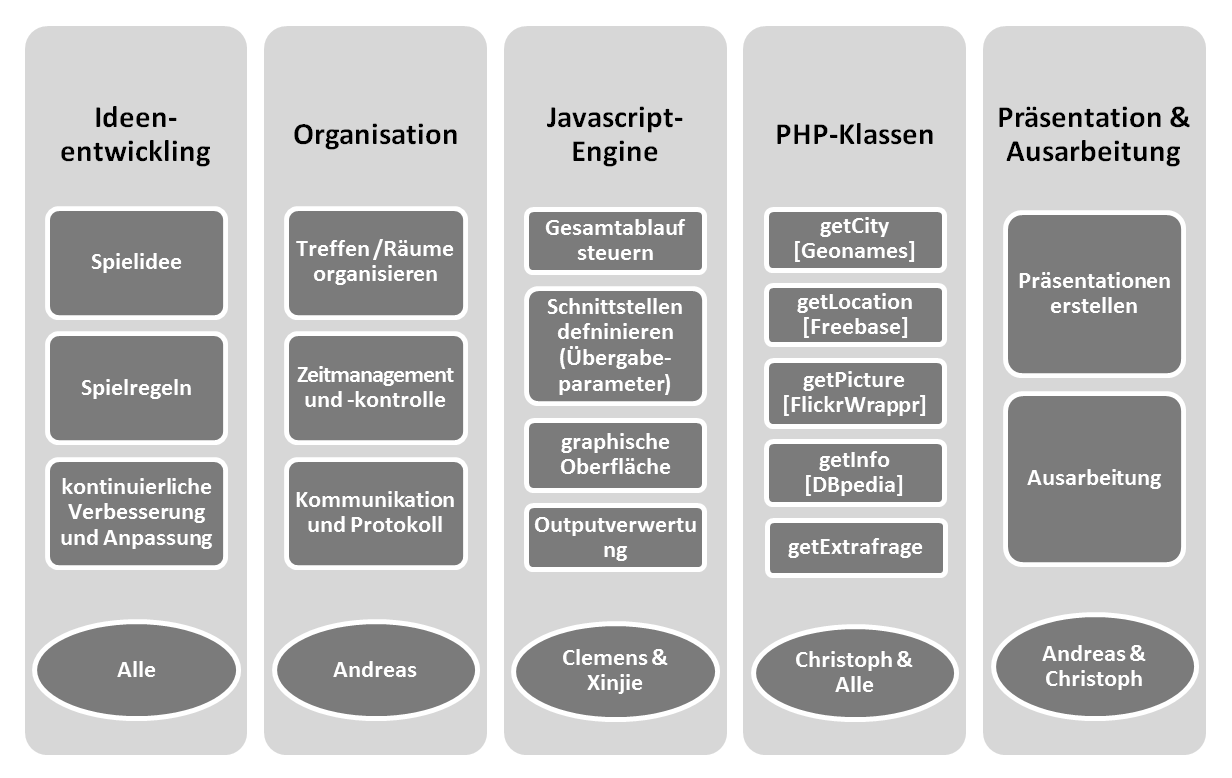
\includegraphics[width=1.0\columnwidth, angle=0]{projektplanung_organigramm_sw.png}
	\caption{Aufteilung der Arbeitspakete}
	\label{pic:Pakete}
\end{figure}
\begin{sidewaysfigure}
	\centering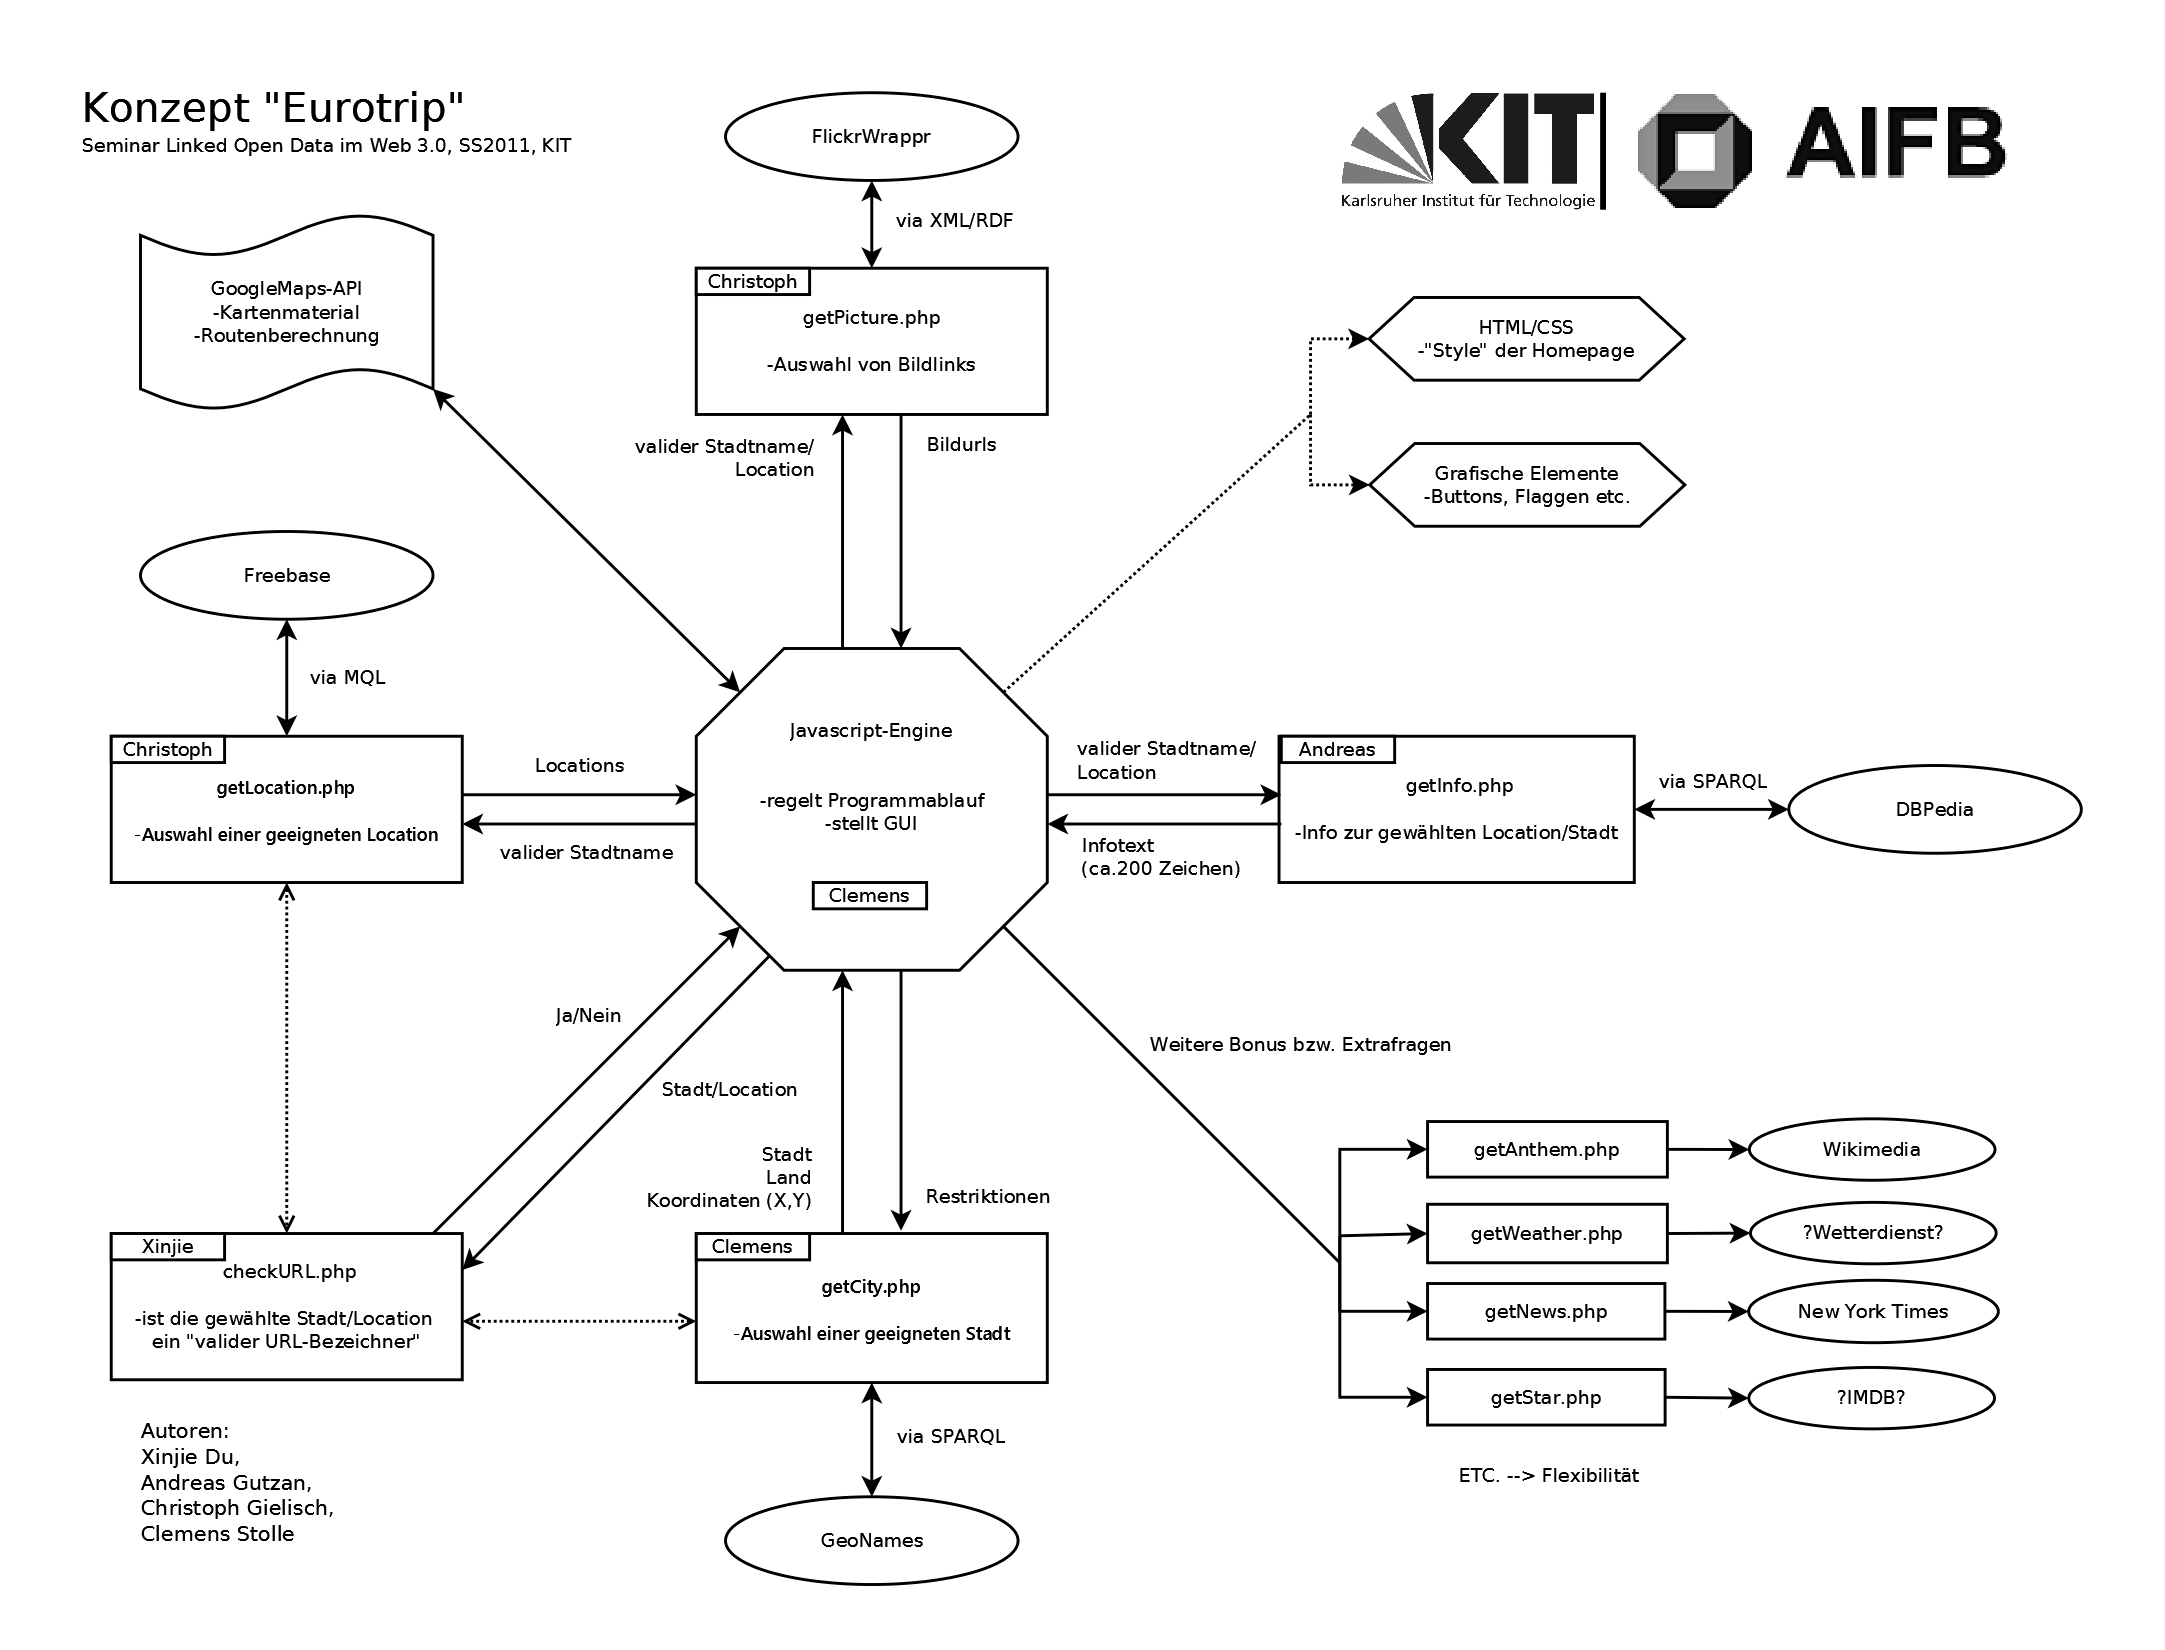
\includegraphics[scale=0.2]{seminarLOD.png}
	\caption{Konzeptskizze Eurotrip}
	\label{pic:Konzept}
\end{sidewaysfigure}
% das ist wohl jetzt das Ende des Dokumentes
\end{document}